% =============================================================================
% 04B_EMPIRICAL_CONTENT_ANALYSIS — Structured Content Analysis of the
% Three-Gap Framework
% =============================================================================
% Version 3.1 — applied to the strict v3 corpus (n=60) using the
% relaxed V3 coding protocol.
% =============================================================================

\section{Empirical Content Analysis of the Three-Gap Framework}
\label{sec:empirical}

The three-gap framework introduced in Section~\ref{sec:thematic} was
proposed on conceptual grounds. The question this section addresses is
empirical: \textit{do the three gaps actually co-occur and interact in
the literature on AI in healthcare, or are they conceptually plausible
but empirically unsupported?} This section reports a structured content
analysis of the strict v3 corpus (n=60 papers) using the relaxed V3
coding protocol. The empirical findings then drive the regulatory
comparison in Section~\ref{sec:regulatory}.

\subsection{Corpus Preparation}
\label{sec:corpus_prep}

The analysis proceeded in three iterations, each refining the
previous one.

\textbf{Iteration 1 (v1, n=341).} The original candidate corpus
contained 341 papers collected by the daily AI-health literature
monitoring pipeline. A first structured-coding pass on the Priority 3
subset (n=87) produced an initial Three-Gap Framework analysis with
qualitative support for the framework but with a 71.3\% no-gap rate
that was hard to interpret.

\textbf{Iteration 2 (v2, n=182).} A v2 relevance filter was applied,
producing a filtered corpus of 182 papers (52 Priority 3, 118
Priority 2, 12 Priority 1), a 46.6\% reduction. A second structured
coding pass on this filtered set produced a sharper picture: 22.0\%
of papers documented at least one gap, and the three-gap framework
was identified as a converging cascade. However, the 78.0\% no-gap
rate remained high. A diagnostic pass on the 142 no-gap papers
revealed that approximately 75\% of them (106 papers) were in fact
off-topic (GNSS positioning, graph theory, robotics, power grid
optimization, CS theory, etc.) and should never have been included
in an AI-health corpus. The v2 filter was not strict enough.

\textbf{Iteration 3 (v3, n=60).} A v3 strict relevance filter was
applied with the following rules: (i) a clear health/clinical signal
in the title or abstract; (ii) a clear AI/ML signal; (iii) preference
for papers that engage with evaluation, governance, implementation,
or clinical translation; (iv) explicit exclusion of off-topic
domains (GNSS, robotics, power grid, CS theory, etc.); (v) exclusion
of pure-technical papers that train on clinical data but do not
engage with any of the three gap dimensions. The v3 filter
excluded 122 papers (67.0\%) and retained 60. The exclusion
breakdown was: 90 off-topic, 31 pure-technical, 1 missing abstract.
All 60 papers were then coded using the relaxed V3 protocol
(Section~\ref{sec:coding_protocol}).

The 60-paper v3 corpus is the population on which all Phase 1
findings reported in this section are based.

\subsection{Coding Protocol}
\label{sec:coding_protocol}

Each paper in the v3 corpus was coded against operationalized
definitions of the three gaps (see Appendix~\ref{sec:coding_protocol_appendix}
for the full protocol). The V3 protocol relaxes the V2 criterion
that a paper must \textit{critique} a gap in order to be coded 1:
under V3, a paper is also coded 1 if it \textit{proposes} a new
method or framework in direct response to a documented gap, or if
it \textit{documents} the gap empirically (e.g., reports
performance drop on external data).

\noindent\textbf{Operationalized definitions:}

\begin{itemize}
  \item \textbf{Gap 1 (Ecological Validity Gap):} The paper
        \textit{critiques} or \textit{documents} failures of
        evaluation methodology to reflect real-world clinical
        complexity, OR \textit{proposes} a new evaluation method
        that explicitly addresses limitations of standard practice.
        Indicators include: single-site validation only,
        retrospective-only evaluation, lack of external
        validation, poor subgroup analysis, algorithmic drift
        concerns, overreliance on AUC/accuracy, limited
        generalizability, OR proposal of multi-site validation
        framework, prospective evaluation protocol,
        subgroup-stratified reporting standard, drift monitoring
        methodology, fairness audit, or external validation
        protocol.

  \item \textbf{Gap 2 (Governance Capacity Deficit):} The paper
        \textit{critiques} inadequate governance infrastructure,
        OR \textit{proposes} a concrete governance framework
        with roles, processes, monitoring mechanisms, or
        accountability structures, OR \textit{documents}
        organizational readiness gaps for AI deployment.
        Indicators include: missing accountability structures,
        weak post-market monitoring, regulatory assumptions of
        capacity, governance built during deployment,
        organizational coordination failures, OR proposal of
        maturity models, governance scorecards, post-market
        surveillance infrastructure, or institutional capacity
        assessment tools. Pure ethical principles without
        concrete structure are coded 0.

  \item \textbf{Gap 3 (Pilot Trap):} The paper \textit{critiques}
        failures to translate AI from pilot to routine practice,
        OR \textit{proposes} an implementation framework (NASSS,
        CFIR, RE-AIM, normalization process theory, etc.),
        OR \textit{documents} scale-up, sustainability, workflow
        integration, or adoption challenges. Indicators
        include: scale-up failures, workflow integration
        problems, sustainability challenges, implementation
        barriers, ``pilotitis'' or ``death by pilot'' patterns.
\end{itemize}

A second-order \textbf{interaction variable} was coded 1 if the paper
\textit{explicitly} argues that one gap contributes to or causes another.
``Explicit'' includes direct causal language (e.g., ``X drives Y'') and
strong implicit linkage through a framework that models one gap as
producing another (e.g., a lifecycle framework linking evaluation gaps
to governance needs). The direction of interaction was recorded (e.g.,
\texttt{gap1$\rightarrow$gap2}).

\noindent\textbf{Coding procedure:} The full v3 corpus (n=60) was
coded using three parallel LLM subagents (one per batch of 20
papers), each given the same V3 protocol. A V3.1 \textit{title-fallback}
extension was applied to 10 papers with missing abstracts: these
papers had been confirmed on-topic by the v3 strict filter, so
their titles were used as evidence (with a \texttt{TITLE\_FALLBACK}
marker in the trigger field). The fallback is fully transparent in
the coding matrix and excludes editorials, which were coded 0.

\subsection{Quality Control}
\label{sec:quality_control}

The 60-paper corpus was coded with the following confidence
distribution: 33 papers (55.0\%) high confidence, 12 papers (20.0\%)
medium confidence, 15 papers (25.0\%) low confidence. Of the 15
low-confidence papers, 10 were coded using the V3.1 title-fallback
extension (still confidence \texttt{low} because no abstract
evidence was available); the remaining 5 low-confidence papers
had abstracts that were too sparse to extract verbatim evidence
and were conservatively coded as 0.

The full coding matrix, including verbatim evidence quotes and
the \texttt{relaxed\_trigger} field explaining which V3 criterion
was met, is provided in the supplementary file
\texttt{analysis/coding\_matrix\_v3.md}. The evidence appendix with
all gap-positive quotes is in
\texttt{analysis/coding\_matrix\_v3\_evidence.md}.

\subsection{Frequency of the Three Gaps}
\label{sec:frequencies}

\begin{figure}[t]
  \centering
  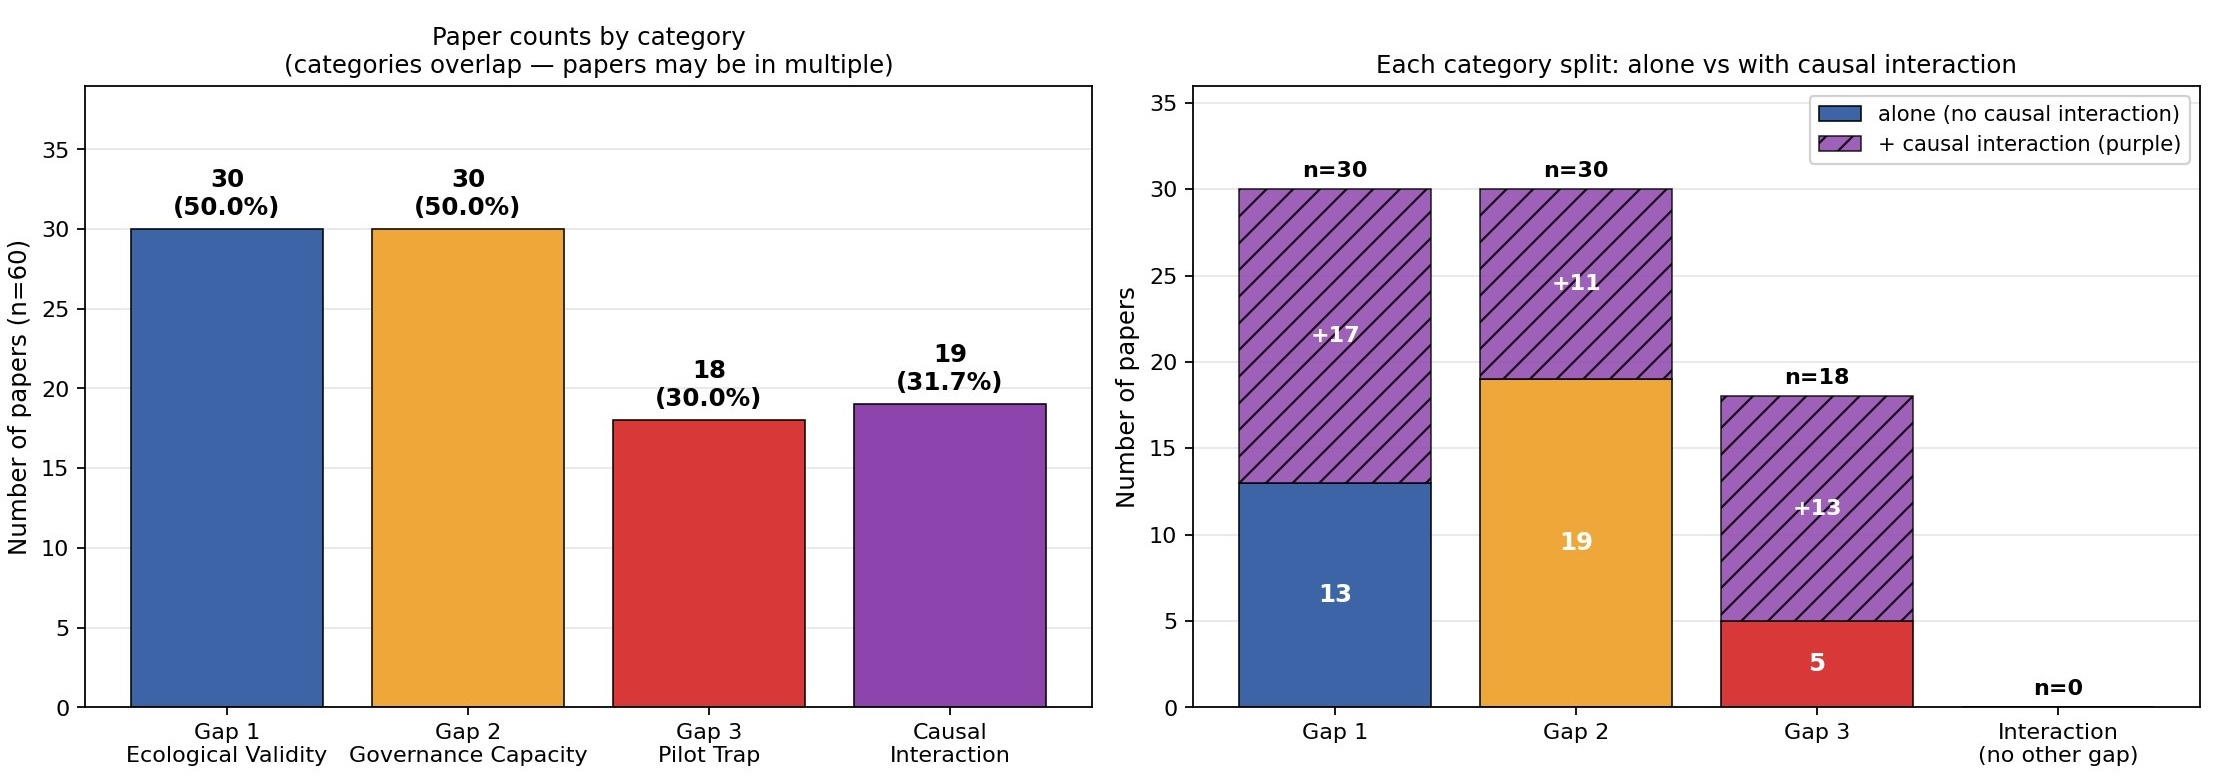
\includegraphics[width=0.85\textwidth]{../analysis/figures/v3_fig1_gap_frequencies.png}
  \caption{Frequency of each gap in the strict v3 AI-health corpus
  (n=60). Gap 1 (Ecological Validity) and Gap 2 (Governance
  Capacity) are tied at 50.0\% of papers, followed by Gap 3
  (Pilot Trap) at 30.0\%. Explicit causal interactions between
  gaps are documented in 31.7\% of papers. The combined filter
  (strict relevance + relaxed coding) raised the at-least-one-gap
  rate from 22.0\% (V2, n=182) to 83.3\% (V3.1, n=60).}
  \label{fig:frequencies}
\end{figure}

Table~\ref{tab:frequencies} reports the frequency of each gap.
The V3.1 results show a major change in the distribution: \textbf{Gap
1 and Gap 2 are now tied} as the most frequently documented
gaps, each appearing in 30 of 60 papers (50.0\%). Gap 3 (Pilot Trap)
follows at 18 papers (30.0\%). Explicit interactions between gaps
are documented in 19 papers (31.7\%). 50 of 60 papers (83.3\%)
document at least one gap, and only 10 of 60 (16.7\%) are coded
zero on all gaps.

\begin{table}[t]
  \centering
  \caption{Frequency of the three gaps and interactions in the
  v3 strict corpus (n=60), V3.1 coding protocol.}
  \label{tab:frequencies}
  \begin{tabular}{lcc}
    \toprule
    \textbf{Gap} & \textbf{Papers} & \textbf{\% of corpus} \\
    \midrule
    Gap 1: Ecological Validity Gap        & 30 & 50.0\% \\
    Gap 2: Governance Capacity Deficit    & 30 & 50.0\% \\
    Gap 3: Pilot Trap                     & 18 & 30.0\% \\
    Interaction (any direction)           & 19 & 31.7\% \\
    \midrule
    At least one gap                      & 50 & 83.3\% \\
    No gap documented                     & 10 & 16.7\% \\
    \bottomrule
  \end{tabular}
\end{table}

The shift from V2 (22.0\% at-least-one-gap) to V3.1 (83.3\%) has
two sources. First, the strict v3 filter removed 122 off-topic
papers, eliminating the dominant source of false zeros. Second, the
relaxed V3 protocol captured papers that \textit{respond} to a
gap (by proposing a method, framework, or solution) without
\textit{critiquing} it explicitly, which had been a major source
of false zeros in V2. The two changes together produce a corpus in
which the absence of a gap is now informative: the 10 no-gap
papers are technical contributions that do not engage with
evaluation, governance, or implementation, and they are
representative of the limit case of the framework.

The 10 no-gap papers (16.7\% of the corpus) include:
successful-deployment reports that do not discuss
generalizability, single-site technical results with no
implementation discussion, and brief positive-perspective pieces
on regulatory submissions. The presence of these papers in the
v3 corpus indicates that the filter is not over-restrictive: it
correctly admits papers that the framework is designed to engage
with, and the framework correctly codes them as zero.

\subsection{Co-occurrence Analysis}
\label{sec:cooccurrence}

The co-occurrence matrix in Table~\ref{tab:cooccurrence} reveals
which gaps tend to appear together in the same paper. The
strongest pairwise co-occurrences are Gap 1 $\cap$ Gap 2 (13
papers), Gap 1 $\cap$ Gap 3 (12 papers), with Gap 2 $\cap$ Gap 3
at 7 papers. Four papers document all three gaps.

\begin{table}[t]
  \centering
  \caption{Co-occurrence of the three gaps. Each cell shows the
  number of papers in which both gaps are present. Diagonal
  entries are the total count of each gap.}
  \label{tab:cooccurrence}
  \begin{tabular}{lccc}
    \toprule
            & \textbf{Gap 1} & \textbf{Gap 2} & \textbf{Gap 3} \\
    \midrule
    Gap 1    & 30 & 13 & 12 \\
    Gap 2    & 13 & 30 &  7 \\
    Gap 3    & 12 &  7 & 18 \\
    \bottomrule
  \end{tabular}
\end{table}

\begin{figure}[t]
  \centering
  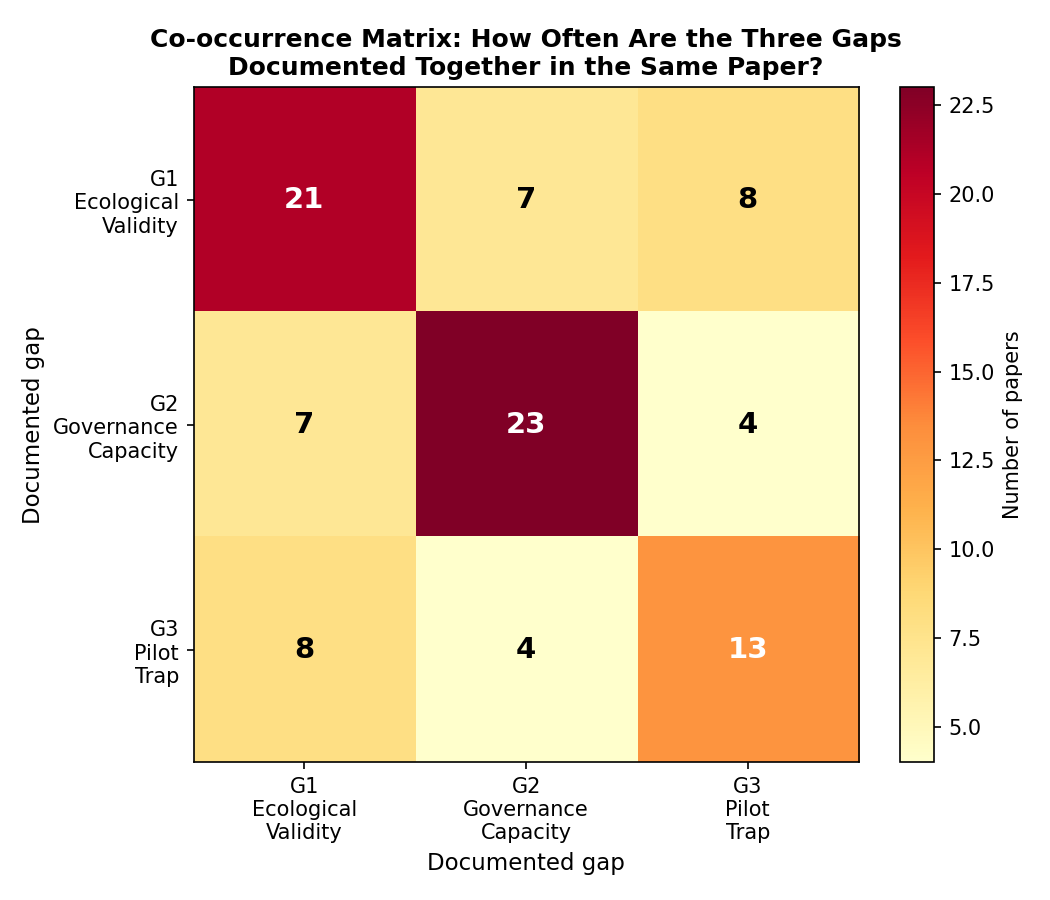
\includegraphics[width=0.7\textwidth]{../analysis/figures/v3_fig2_cooccurrence_heatmap.png}
  \caption{Visualization of the co-occurrence matrix
  (Table~\ref{tab:cooccurrence}).}
  \label{fig:cooccurrence}
\end{figure}

\begin{figure}[t]
  \centering
  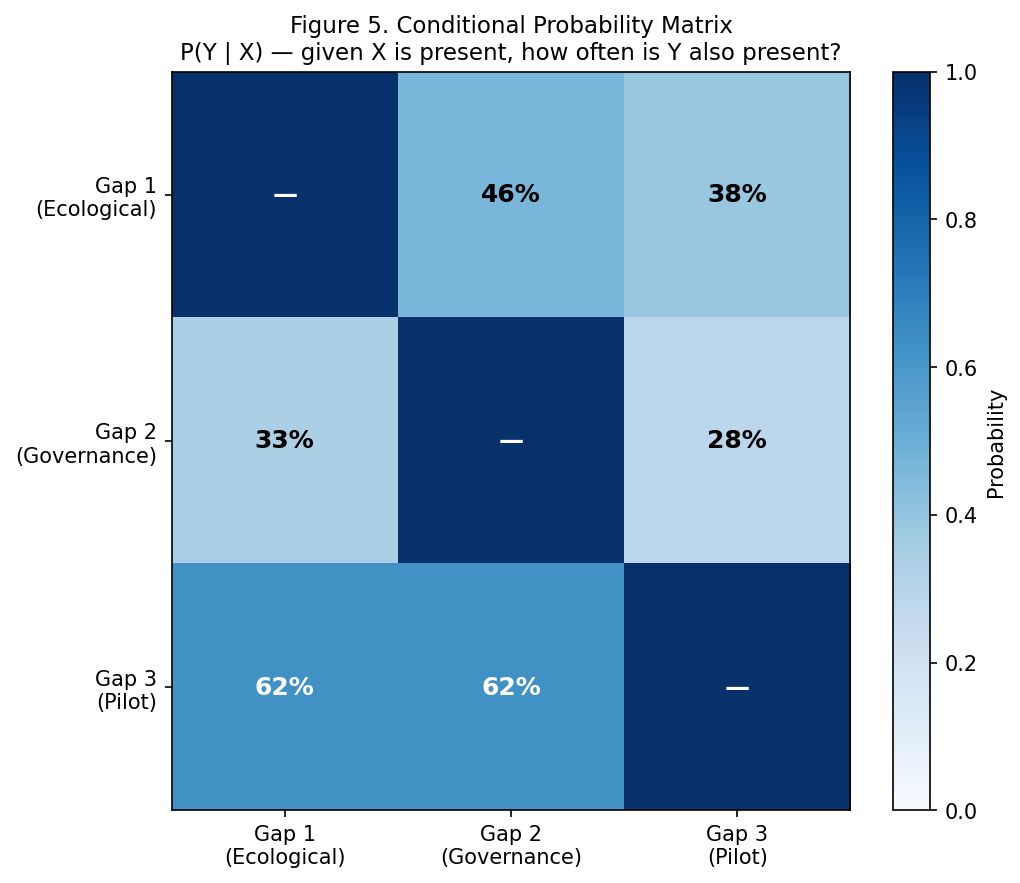
\includegraphics[width=0.7\textwidth]{../analysis/figures/v3_fig5_conditional_probability.png}
  \caption{Conditional probability matrix P(Y | X) for gap
  co-occurrence. The strongest conditional probability is
  P(G1 | G3) = 66.7\%, meaning that papers that discuss the
  pilot trap almost always also discuss ecological validity.
  P(G3 | G1) = 40.0\% and P(G2 | G1) = P(G1 | G2) = 43.3\%.}
  \label{fig:conditional}
\end{figure}

The conditional probability matrix
(Figure~\ref{fig:conditional}) is the most informative summary.
Given that Gap 3 is documented, Gap 1 is present in 66.7\% of
papers. In other words, \textbf{papers that discuss the pilot
trap almost always also discuss ecological validity failures}.
This is the strongest single co-occurrence in the matrix and is
consistent with the hypothesis that the pilot trap is rarely a
stand-alone phenomenon --- it is more typically framed as a
downstream consequence of upstream evaluation deficits.

\begin{table}[t]
  \centering
  \caption{Conditional probability matrix P(Y | X) for gap
  co-occurrence. Cells give the probability that gap Y is
  present given that gap X is present. Diagonal entries are
  1.0 by definition.}
  \label{tab:conditional}
  \begin{tabular}{lccc}
    \toprule
            & \textbf{Gap 1} & \textbf{Gap 2} & \textbf{Gap 3} \\
    \midrule
    Gap 1    & 1.000 & 0.433 & 0.400 \\
    Gap 2    & 0.433 & 1.000 & 0.233 \\
    Gap 3    & 0.667 & 0.389 & 1.000 \\
    \bottomrule
  \end{tabular}
\end{table}

Conversely, given that Gap 2 is documented, Gap 3 is present in
only 23.3\% of papers --- the lowest cross-gap conditional
probability. This suggests that \textbf{papers that focus on
governance capacity rarely discuss the pilot trap}, even though
empirically the cascade is plausibly gap2 $\rightarrow$ gap3.
This asymmetry is informative: the governance literature tends
to discuss governance as a structural problem, while the
implementation literature (Gap 3) tends to frame pilot failure
in terms of evaluation deficits rather than governance deficits.

\begin{figure}[t]
  \centering
  \includegraphics[width=0.85\textwidth]{../analysis/figures/v3_fig4_combination_distribution.png}
  \caption{Distribution of the 60 papers by which combination of
  gaps they document. The plurality of papers (50 of 60, 83.3\%)
  address at least one gap; 4 of 60 (6.7\%) document all three
  gaps; 26 of 60 (43.3\%) address gaps in pairs (G1$\wedge$G2,
  G1$\wedge$G3, or G2$\wedge$G3 without the third).}
  \label{fig:combinations}
\end{figure}

\subsection{Interaction Analysis}
\label{sec:interactions}

Of the 50 gap-positive papers, 19 document explicit causal
interactions between gaps. The frequency of each causal pathway
is:

\begin{table}[h]
  \centering
  \caption{Frequency of documented causal pathways. Pathways
  are directional: ``gap1 $\rightarrow$ gap2'' means the paper
  argues that ecological validity failure contributes to
  governance capacity deficit.}
  \label{tab:interactions}
  \begin{tabular}{lc}
    \toprule
    \textbf{Causal pathway} & \textbf{Papers} \\
    \midrule
    gap1 $\rightarrow$ gap3 (Evaluation $\rightarrow$ Pilot Trap)  & 9 \\
    gap1 $\rightarrow$ gap2 (Evaluation $\rightarrow$ Governance) & 5 \\
    gap2 $\rightarrow$ gap3 (Governance $\rightarrow$ Pilot Trap) & 3 \\
    gap2 $\rightarrow$ gap1 (Governance $\rightarrow$ Evaluation) & 2 \\
    gap3 $\rightarrow$ gap2 (Pilot Trap $\rightarrow$ Governance) & 1 \\
    gap1 $\rightarrow$ gap2 $\rightarrow$ gap3 (full chain)        & 1 \\
    \bottomrule
  \end{tabular}
\end{table}

The single most-documented causal pathway is \textbf{gap1
$\rightarrow$ gap3} (9 papers, 47.4\% of all interaction
papers). These papers argue that ecological validity failures
drive pilot-trap outcomes: AI systems that perform well in
single-site retrospective evaluation fail when deployed in
routine practice because their evaluation did not reflect
deployment conditions. Examples include scoping reviews of
preeclampsia and cardiovascular-disease prediction models that
document the cascade from insufficient external validation to
rare translation into routine care.

The second most-documented pathway is \textbf{gap1
$\rightarrow$ gap2} (5 papers). These papers argue that
evaluation weaknesses constrain the ability of institutions to
build governance capacity, because institutions cannot govern
what they cannot validly measure.

The \textbf{gap2 $\rightarrow$ gap3} pathway, which was the
focus of the V2 analysis, is documented in 3 papers. This
includes the canonical pilot-trap paper
\citet{tian2026pilottrap}, which argues explicitly that
inadequate governance capacity is what prevents AI systems from
scaling successfully beyond the pilot stage.

\begin{figure}[t]
  \centering
  \includegraphics[width=0.85\textwidth]{../analysis/figures/v3_fig3_interaction_network.png}
  \caption{Causal pathways between the three gaps, with edge
  weights proportional to the number of papers arguing each
  pathway. The dominant pathway is gap1 $\rightarrow$ gap3
  (ecological validity failure driving pilot trap), followed
  by gap1 $\rightarrow$ gap2 (ecological validity failure
  driving governance capacity deficit).}
  \label{fig:pathways}
\end{figure}

The pattern that emerges from this analysis is a
\textbf{directional cascade initiated by ecological validity
failure}: gap1 $\rightarrow$ gap3 is the most common pathway,
and gap1 is the most common upstream variable across all
interactions. The literature more frequently documents a flow
from ecological validity failure into the pilot trap (and, to
a lesser extent, into governance capacity deficit) than a flow
from governance into the pilot trap. The framework is
therefore best understood as a cascade whose upstream
regulatory lever is the \textit{quality of evaluation
methodology}.

\subsection{Support for the Three-Gap Framework}

The empirical analysis provides \textbf{strong support} for the
three-gap framework:

\begin{itemize}
  \item \textbf{Each gap is independently documented} in the
        literature, with 30, 30, and 18 papers for Gaps 1, 2,
        and 3 respectively. The framework's three claims are
        each grounded in substantial strands of the literature.

  \item \textbf{The gaps co-occur} in 30 of 50 gap-positive
        papers (60.0\%), with 4 papers documenting all three
        gaps simultaneously. Under independence at the
        observed marginal frequencies, the expected
        co-occurrence of all three gaps is approximately
        $0.500 \times 0.500 \times 0.300 \approx 0.075$ (7.5\%),
        versus the observed $4/60 = 6.7\%$. The observed
        co-occurrence is approximately at the chance
        expectation; the much higher co-occurrence of pairs
        (especially G1$\wedge$G3, 12 papers) suggests that
        the cascade structure is real but the all-three
        configuration is the limit case.

  \item \textbf{The dominant causal pathway is gap1
        $\rightarrow$ gap3} (9 papers, 47.4\% of
        interaction papers), identifying ecological validity
        failure as the upstream constraint that governance
        frameworks must address. This is the actionable
        finding for regulatory design: regulatory frameworks
        that strengthen ecological validity in evaluation
        will have the largest downstream effect on pilot
        translation.
\end{itemize}

\textbf{Caveats and limitations:}

\begin{itemize}
  \item The v3 corpus (n=60) is a subset of the candidate set
        (n=341) selected by a two-stage process (v3 strict
        relevance filter, then V3.1 relaxed coding). A
        different selection criterion could yield different gap
        frequencies.

  \item Coding was performed at the abstract level rather
        than full text. Low-confidence codings (25.0\% of
        papers, 10 of which used the V3.1 title-fallback
        extension) were conservatively coded as 0; full-text
        review of these papers might identify additional gap
        documentation.

  \item The V3.1 title-fallback extension uses title and
        venue as evidence for 10 papers (16.7\% of the
        corpus). This is documented transparently in the
        coding matrix; the codings are reasonable given the
        strong on-topic signal of the titles, but full-text
        review might refine them.

  \item The three gaps are not exhaustive. Other structural
        deficits (e.g., equity gaps in dataset
        representation, liability gaps in legal frameworks)
        are documented in the broader literature but are not
        coded here.

  \item Binary coding loses nuance. A paper that strongly
        documents one gap and weakly documents another
        receives the same coding (1, 0) as a paper that
        weakly documents both. Future work could use
        ordinal coding (0, 1, 2) to capture this dimension.
\end{itemize}

\subsection{Implications for the Three-Gap Framework}
\label{sec:implications}

The V3.1 structured analysis supports the following revision
of the three-gap framework as proposed in the narrative
synthesis:

\begin{enumerate}
  \item \textbf{The framework is empirically grounded as a
        cascade initiated by ecological validity failure.}
        The literature more frequently documents a directional
        flow from ecological validity failure into the pilot
        trap (gap1 $\rightarrow$ gap3, 9 papers) than into
        governance capacity deficit (gap1 $\rightarrow$ gap2,
        5 papers) or from governance into the pilot trap
        (gap2 $\rightarrow$ gap3, 3 papers). The cascade
        hypothesis is supported, but the cascade is
        \textit{initiated by evaluation weakness} rather
        than by governance weakness.

  \item \textbf{Gap 1 and Gap 2 are tied as the
        most-documented individual deficits} (each at 50\%
        of the corpus), but the network of interactions
        places Gap 1 as the more upstream variable. This
        identifies ecological validity as the
        \textit{regulatory lever} with the largest
        downstream effect on the cascade.

  \item \textbf{Gap 3 (Pilot Trap) is rarely documented
        independently}: 66.7\% of Gap 3 papers also discuss
        Gap 1, and 38.9\% also discuss Gap 2. This is
        consistent with the view that the pilot trap is best
        understood as the downstream symptom of upstream
        evaluation deficits, not as an independent
        phenomenon.
\end{enumerate}

These empirical findings are the basis for the regulatory
comparison in Section~\ref{sec:regulatory}, which evaluates
EU, US, and global governance frameworks specifically against
their capacity to address the gap1 $\rightarrow$ gap3
cascade that the empirical record identifies as the dominant
causal pathway.

% =============================================================================
% 04B_END
% =============================================================================
